% !TEX TS-program = pdflatex
% !TEX encoding = UTF-8 Unicode

% This is a simple template for a LaTeX document using the "article" class.
% See "book", "report", "letter" for other types of document.

\documentclass[11pt]{article} % use larger type; default would be 10pt

\usepackage[utf8]{inputenc} % set input encoding (not needed with XeLaTeX)

%%% Examples of Article customizations
% These packages are optional, depending whether you want the features they provide.
% See the LaTeX Companion or other references for full information.

%%% PAGE DIMENSIONS
\usepackage{geometry} % to change the page dimensions
\geometry{a4paper} % or letterpaper (US) or a5paper or....
% \geometry{margin=2in} % for example, change the margins to 2 inches all round
% \geometry{landscape} % set up the page for landscape
%   read geometry.pdf for detailed page layout information

\usepackage{graphicx} % support the \includegraphics command and options

% \usepackage[parfill]{parskip} % Activate to begin paragraphs with an empty line rather than an indent

%%% PACKAGES
\usepackage{booktabs} % for much better looking tables
\usepackage{array} % for better arrays (eg matrices) in maths
\usepackage{paralist} % very flexible & customisable lists (eg. enumerate/itemize, etc.)
\usepackage{verbatim} % adds environment for commenting out blocks of text & for better verbatim
\usepackage{subfig} % make it possible to include more than one captioned figure/table in a single float
% These packages are all incorporated in the memoir class to one degree or another...

%%% HEADERS & FOOTERS
\usepackage{fancyhdr} % This should be set AFTER setting up the page geometry
\pagestyle{fancy} % options: empty , plain , fancy
\renewcommand{\headrulewidth}{0pt} % customise the layout...
\lhead{}\chead{}\rhead{}
\lfoot{}\cfoot{\thepage}\rfoot{}

%%% SECTION TITLE APPEARANCE
\usepackage{sectsty}
\allsectionsfont{\sffamily\mdseries\upshape} % (See the fntguide.pdf for font help)
% (This matches ConTeXt defaults)

%%% ToC (table of contents) APPEARANCE
\usepackage[nottoc,notlof,notlot]{tocbibind} % Put the bibliography in the ToC
\usepackage[titles,subfigure]{tocloft} % Alter the style of the Table of Contents
\renewcommand{\cftsecfont}{\rmfamily\mdseries\upshape}
\renewcommand{\cftsecpagefont}{\rmfamily\mdseries\upshape} % No bold!

%%% END Article customizations

%%% The "real" document content comes below...

\title{Lecture 15}
\author{TLS and secure channels}
%\date{} % Activate to display a given date or no date (if empty),
         % otherwise the current date is printed 

\begin{document}
\maketitle

\section{Common Crytographic Network Protocols}

\subsection{TLS (Transport Layer Security)}
\begin{itemize}
  \item  Used to provide an encryption wrapper around HTTP to make HTTPS, and for
  many other application layer protocols.
  \item TLS is wrapped around the application layer.
  \item Security goals: Authenticate server, confidentiality and integrity of
  traffic. Ensure that client is connected to the server they think they are
  connected to.
  \item Originally called the Secure Socket Layer (SSL).
\end{itemize}

\subsection{SSH (Secure Shell)}
\begin{itemize}
  \item Encrypted alternative to Telnet, Telnet uses an unencrypted connection
  that sends information in plaintext, which is easily exploitable.
  \item Security goals: Authenticate server and client, confidentiality and
  integrity of traffic.
\end{itemize}

\subsection{IPsec (Internet Protocol Security)}
\begin{itemize}
  \item Provides an encrypted, authenticated alternative to IP. Complicated set
  of protocols which attempt to replace the IP layer.
  \item Regular IP is insecure because anyone can view the payload of packets.
  \item Tunnel IPSec through IP.
  \item Commonly used for VPNs (Virtual Private Networks).
  \item Security goals: client and server authentication, authenticate headers,
  optionally encrypt headers, ensure confidentiality and integrity of payloads.
\end{itemize}

\section{Constructing a Secure Encrypted Channel}
To construct a secure encrypted channel there are several steps of prelinary
communication that the client and server must perform before the channel can be
established.

\subsection{Encrypt and MAC data}

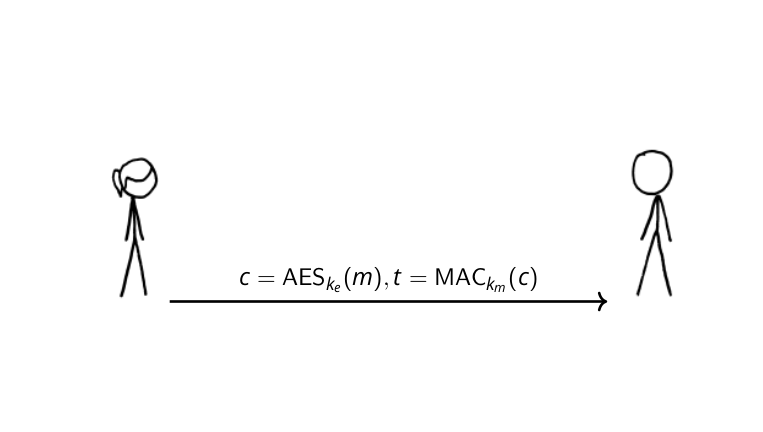
\includegraphics[scale=.7]{./tls1.png}

{\parindent0pt Alice[left] and Bob[right] want to communicate on a secure 
channel on that is protected against passive easedroppers and man-in-the-middle
attacks.}

\bigskip
{\parindent0pt Assuming Alice and Bob have shared a set of keys, Alice sends her
AES ciphertext and the MAC of the ciphertext to Bob.  Bob can now check the MAC
and decrypt the cipher text to get the original message.}

\newpage
\subsection{Diffie-Hellman key exchange}
In order to negotiate charing encryption and MAC keys, there must be a
Diffie-Hellman key exchange.

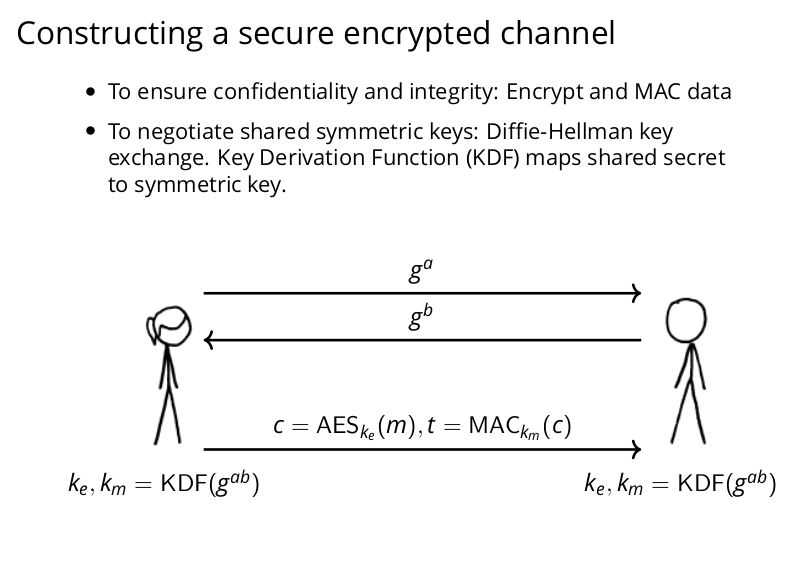
\includegraphics[scale=.7]{./tls2.png}

{\parindent0pt \textbf{NOTE:} In the image above $g^{a}$  should be read as 
$g^{a}\ mod\ p$ and likewise $g^{b}$ should be read $g^{b}\ mod\ p$}

\bigskip
{\parindent0pt If a Diffie-Hellman key exchange has occurred then both Alice 
and Bob will have a \textbf{shared secret}. In this case Alice and Bob's shared
secret is $g^{ab}$.}

\bigskip
{\parindent0pt Using this shared secret Bob and Alice can use a Key Derivation
Function (KDF), 
\smallskip
$k_e, k_m\ =\ KDF(g^{ab})$, which we can think of as a hash function that is 
used to create encryption and MAC keys they can use for symmetric crypto.}

\newpage
\subsection{Ensure Authenticity of Endpoints}
There is a vulnerabiliy with this approach because if there is an active
man-in-the-middle attack, they could man-in-the-middle attack the Diffie-Hellman
key exchange.  To ensure the authenticity of the endpoint we must use
\textbf{digital signatures}, to prevent man-in-the-middle interference of the
key exchange.
\smallskip
You can either have one or both parties sign the key exchange with a long-term
public key.

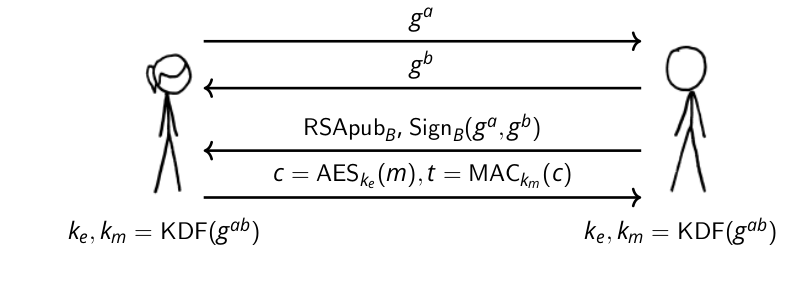
\includegraphics[scale=.7]{./tls3.png}

For the sake of example, assume that Alice is the client [web browser], Bob is 
the web server, Alice knows the server's long-term key, and Alice is trying to
communicate with Bob.

\bigskip
To protect the Diffie-Hellman key exchange Bob will sign the key exchange with 
his long-term key.  Since Alice knows both Bob's original long term-key and the
signature which Bob has given Alice can verify the signature by using Bob's
public key before progressing with the encryption.

\newpage
\subsection{Trusting Signatures}
While we may now be protected against man-in-the-middle attacks targeted towards
the Diffie-Hellman key exchange, we have still not verified the integrity of
Bob's public signing key which Alice has received.

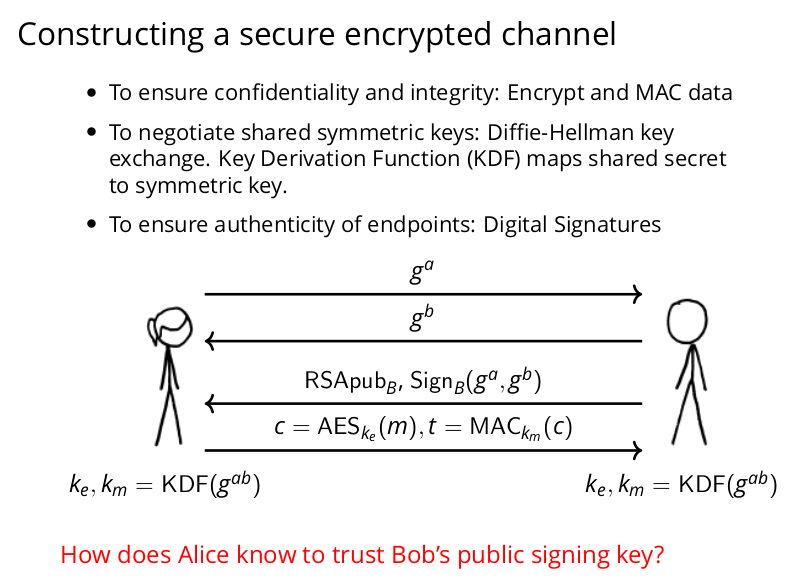
\includegraphics[scale=.7]{./tls4.png}

The public signing key that Bob sends to Alice is susceptible to
active man-in-the-middle attacks, so we must determine a way to trust the keys 
the client receives.

\bigskip
Assuming that there was a man-in-the-middle who was overseeing all the
communications between Alice and Bob, an attacker could substitute Bob's public
key with their own generated public key and Alice would not be able to tell 
the difference.

\bigskip
Due to the nature of this attack, we must have an \textbf{external} method of
establishing trust in keys.

\newpage
\subsection{Establishing Trust in Keys}
TODO

\newpage
\section{TSL: Transport Layer Security}

\subsection{TSL Overview}

\newpage
\subsection{TLS 1.2 with Diffie-Hellman Key Exchange}

\subsubsection{Step 1}
Step 1 of TLS 1.2 with a Diffie-Hellman Key Exchange is 

\newpage
\subsubsection{Step 2}
Step 2 of TLS 1.2 with a Diffie-Hellman Key Exchange is 

\newpage
\subsubsection{Step 3}
Step 3 of TLS 1.2 with a Diffie-Hellman Key Exchange is the server sends over 
its certificate, which contains the server’s public RSA key and a certificate 
authority's signatures.\\

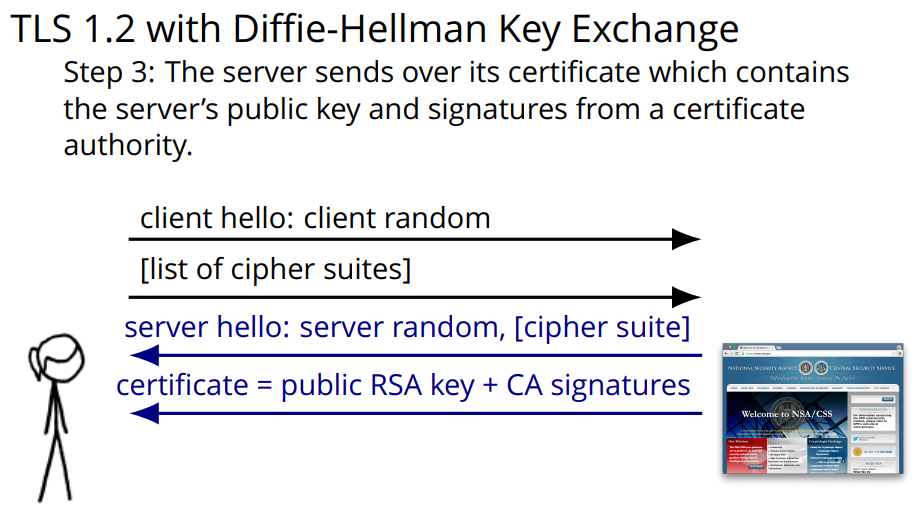
\includegraphics[scale=.8]{./DiffieStep3.png}

(Certificates are explained more in Section 3.3)

\subsubsection{Step 4}
Step 4 of TLS 1.2 with a Diffie-Hellman Key Exchange is the server starts the 
key exchange.\\

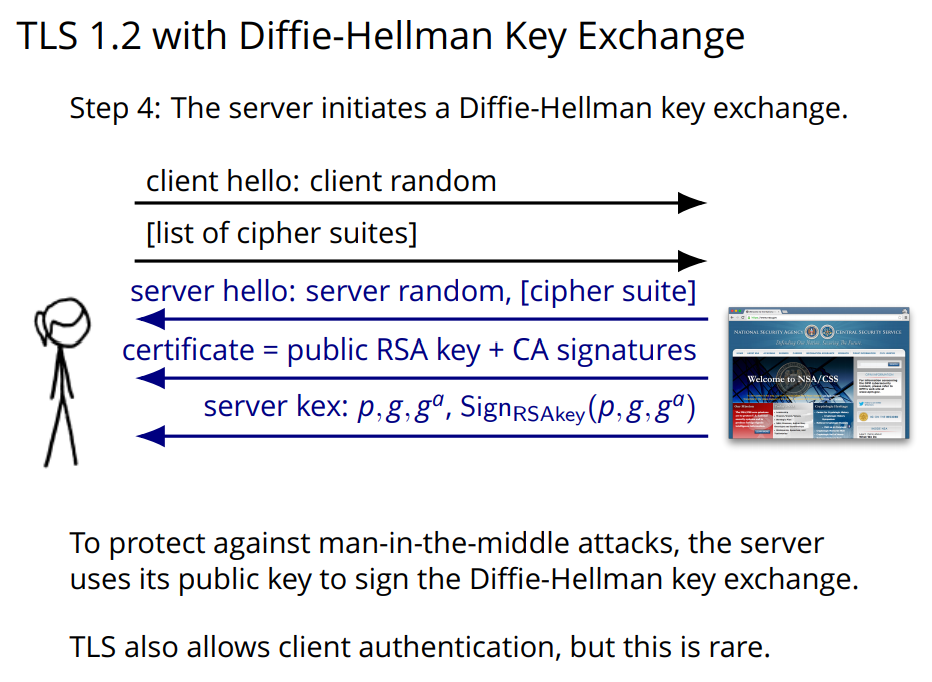
\includegraphics[scale=.8]{./DiffieStep4.png}

 The server will sign its part of the key exchange, shown as 
 $Sign_{RSAkey}(p,g,g^a)$ in the image above. Since the message is signed by 
 the server's RSA key, which is signed by a certificate authority that Alice 
 trusts, it cannot be modified by a man-in-the-middle attacker.

\newpage
\subsubsection{Step 5}
Step 5 of TLS 1.2 with a Diffie-Hellman Key Exchange is Alice[client] does her 
part of the key exchange. \\

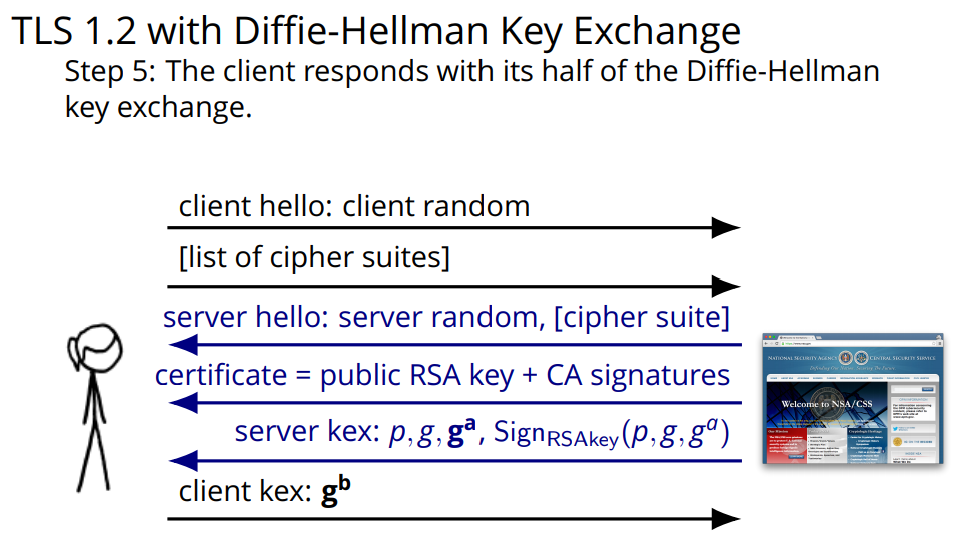
\includegraphics[scale=.8]{./DiffieStep5.png}

This message is usually not authenticated since user authentication is not 
commonly done at the cryptographic layer when using the web.

\subsubsection{Step 6}
Step 6 of TLS 1.2 with a Diffie-Hellman Key Exchange is for the client and 
server to derive the symmetric encryption keys. This is done using a key 
derivation function. \\

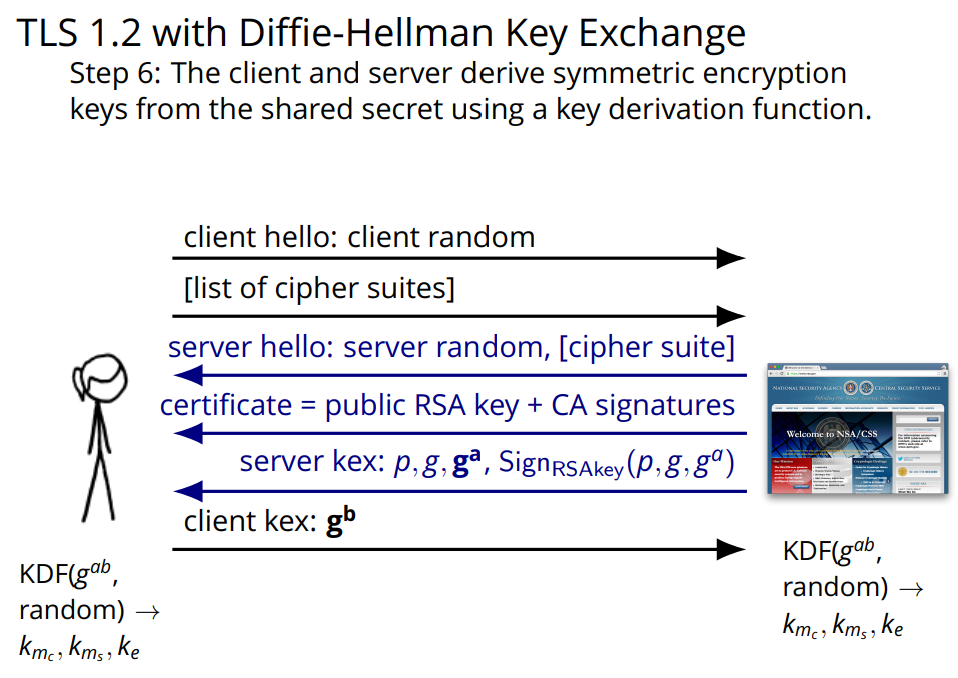
\includegraphics[scale=.8]{./DiffieStep6.png}

$KDF$ in the image above stands for key derivation function.

$k_{m_c}$, $k_{m_s}$, and $k_{e}$ are the symmetric keys.

$k_{m_c}$ is the client's MAC key. $k_{m_s}$ is the server's MAC key. $k_{e}$ 
is the encryption key.

\newpage
\subsubsection{Step 7}
Step 7 of TLS 1.2 with a Diffie-Hellman Key Exchange is for the client and 
server to makes sure that messages were not changed by a man-in-the-middle 
attacker. \\

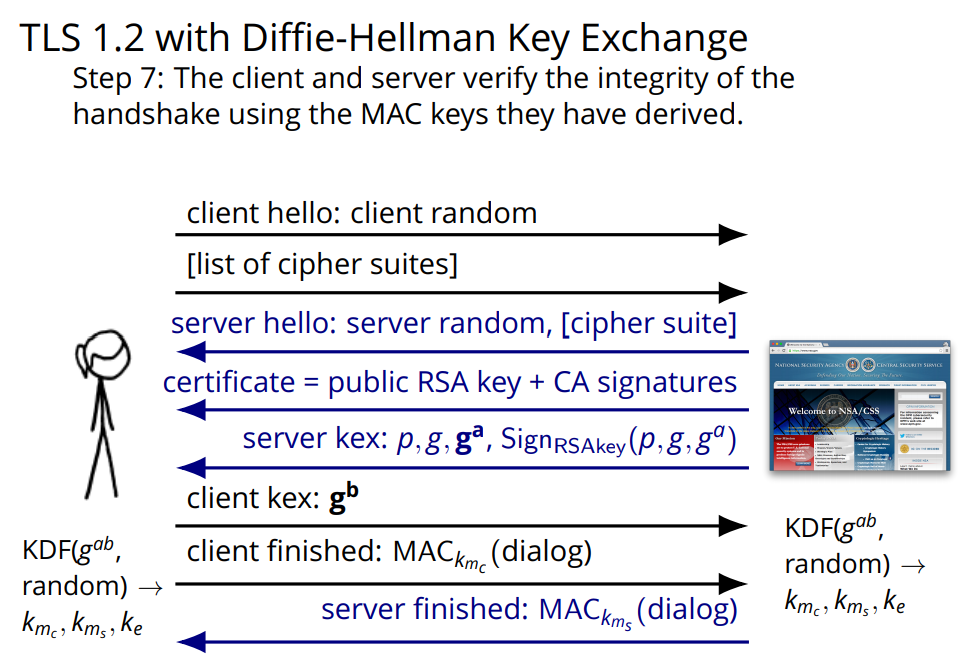
\includegraphics[scale=1.2]{./DiffieStep7.png}
\\

They can verify the integrity of the handshake by each sending a MAC (Message 
Authentication Code) of all of the messages they have sent so far using the 
symmetric keys that they derived in the last step.

They will then be sure that the protocol has not been changed.

\newpage
\subsubsection{Step 8}
Step 8, the last step, of TLS 1.2 with a Diffie-Hellman Key Exchange is to 
send symmetrically encrypted requests. \\

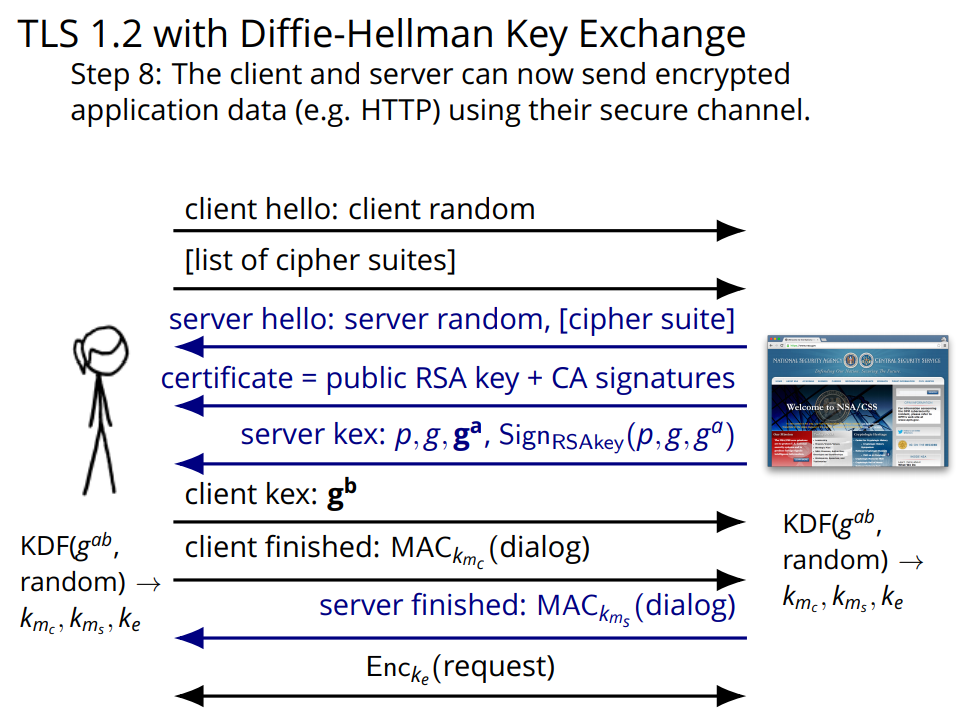
\includegraphics[scale=1.2]{./DiffieStep8.png}
\\

For example, Alice[client] will make a HTTP GET request for index.html over 
the encrypted channel.

\newpage
\subsection{Certificates and Certificate Authorities in TLS}

\subsection{Revocation}

\subsection{Root CAs on OS X}

\subsection{Man-in-the-Middle Attack Using Rogue Cert}

\newpage
\subsection{TLS 1.2 with RSA Key Exchange}
Another way to negotiate keys in TLS 1.2 is using RSA public key encryption to 
share a secret master key.

\begin{enumerate}
  \item This starts with the Alice[client] sending a hello.
  \item Then, the server will send over its certificate, which contains its 
  public key.
  \item Alice[client] will choose a random value, called a premaster secret, 
  which she encrypts to the server's RSA public key and sends back to the 
  server.
  \item The server is the only one who can decrypt the value of the encrypted 
  premaster secret.
  \item The server and client will then use a key derivation function to 
  derive their encryption and MAC keys.
  \item The server and client will exchange MACs of the dialogue.
  \item Finally, they will send encrypted requests using the symmetric 
  encryption key.
\end{enumerate}

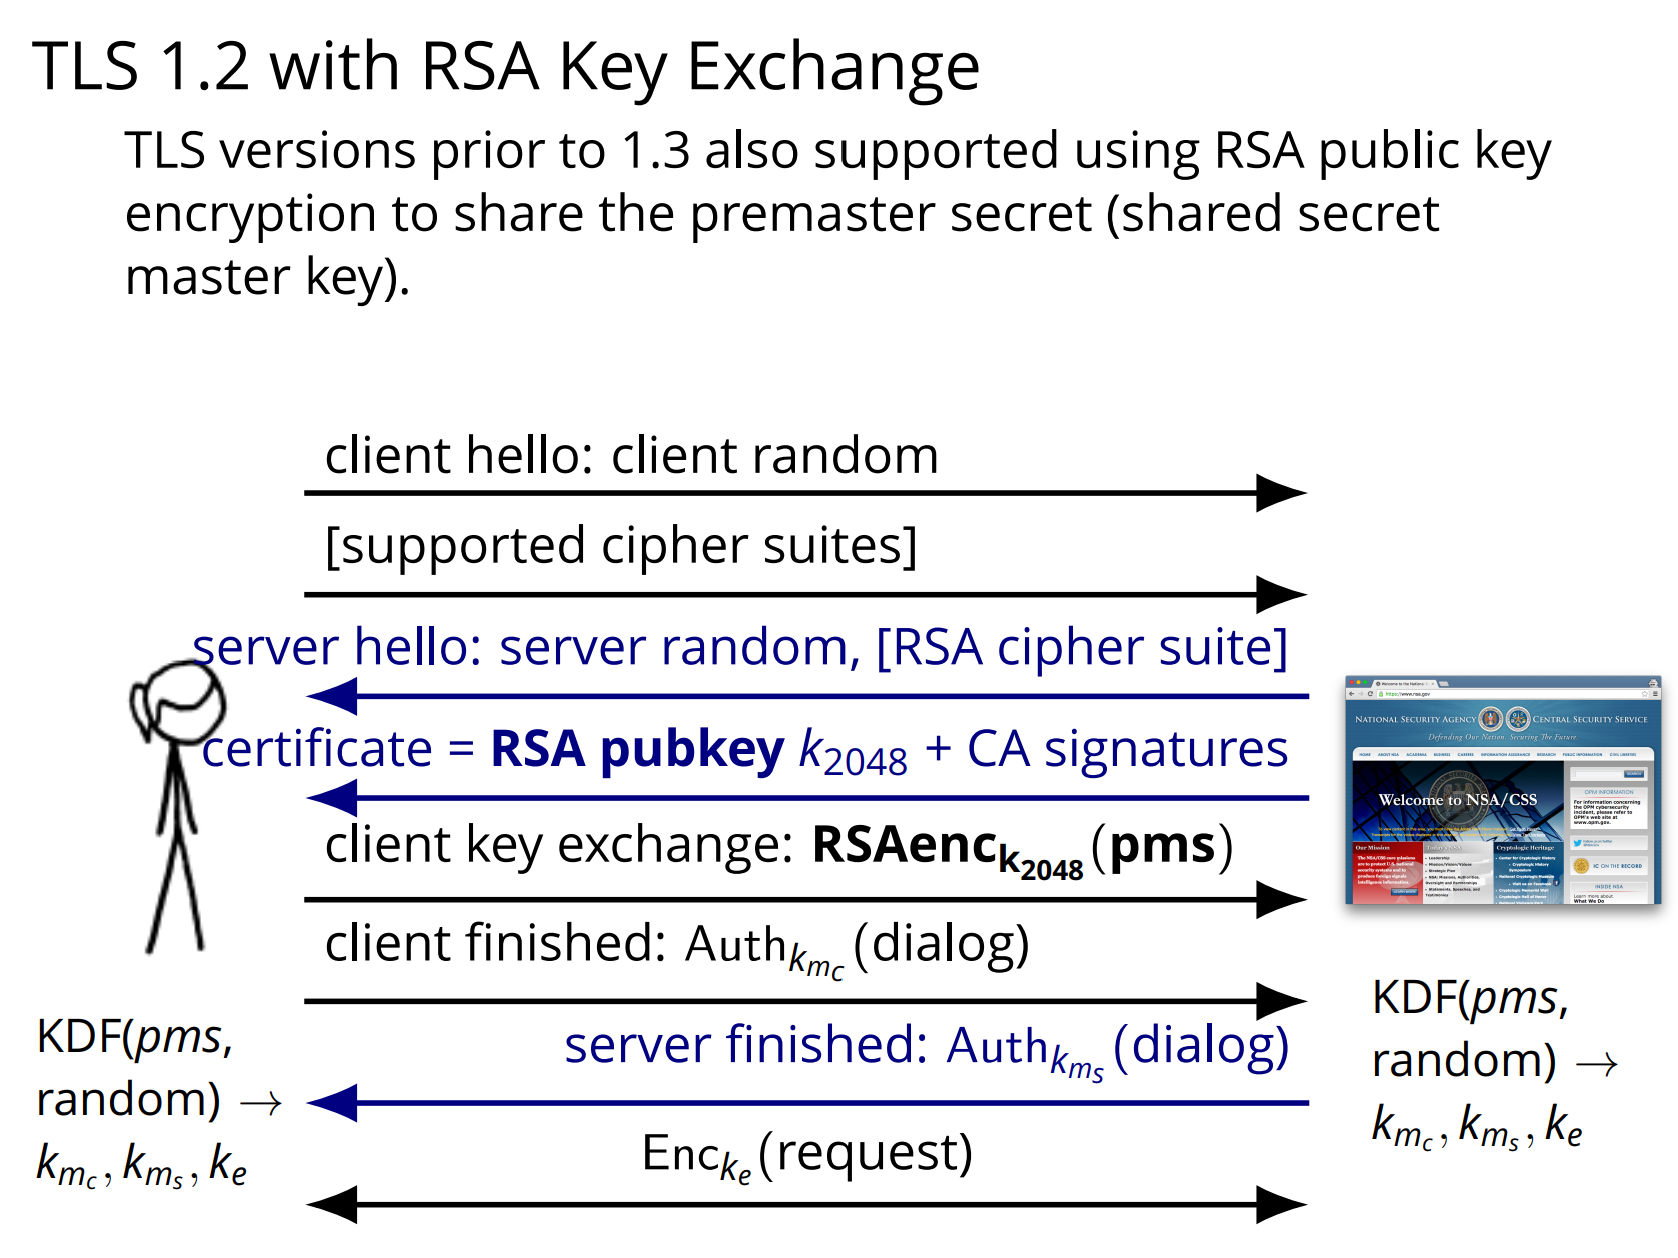
\includegraphics[scale=.6]{./TLS_RSA.png}

The only difference from using the Diffie-Hellman key exchange is the client 
instead encrypts a secret and sends it to the server.

\newpage
\subsection{How TLS Achieves Its Security Goals}

\subsection{What If a Private Key Gets Stolen or Compromised?}

\subsection{TLS v. 1.2 and Below Vulnerabilities}

\subsection{TLS 1.3}

\subsection{TLS Key Theft and Other Risks in the Wild (not in lecture)}

\subsection{The “Crypto Wars” and the Historical Development of TLS (not in 
lecture)}

Even if TLS and key exchange works perfectly, there is still the matter of old-fashioned extortion by powerful governments. Consider, for example, the events of 2013, after Edward Snowden blew the whistle on the NSA's domestic spying capabilities.

Snowden was using a secure mail service Lavabit. In order for the US government to spy on his communications after his defection.

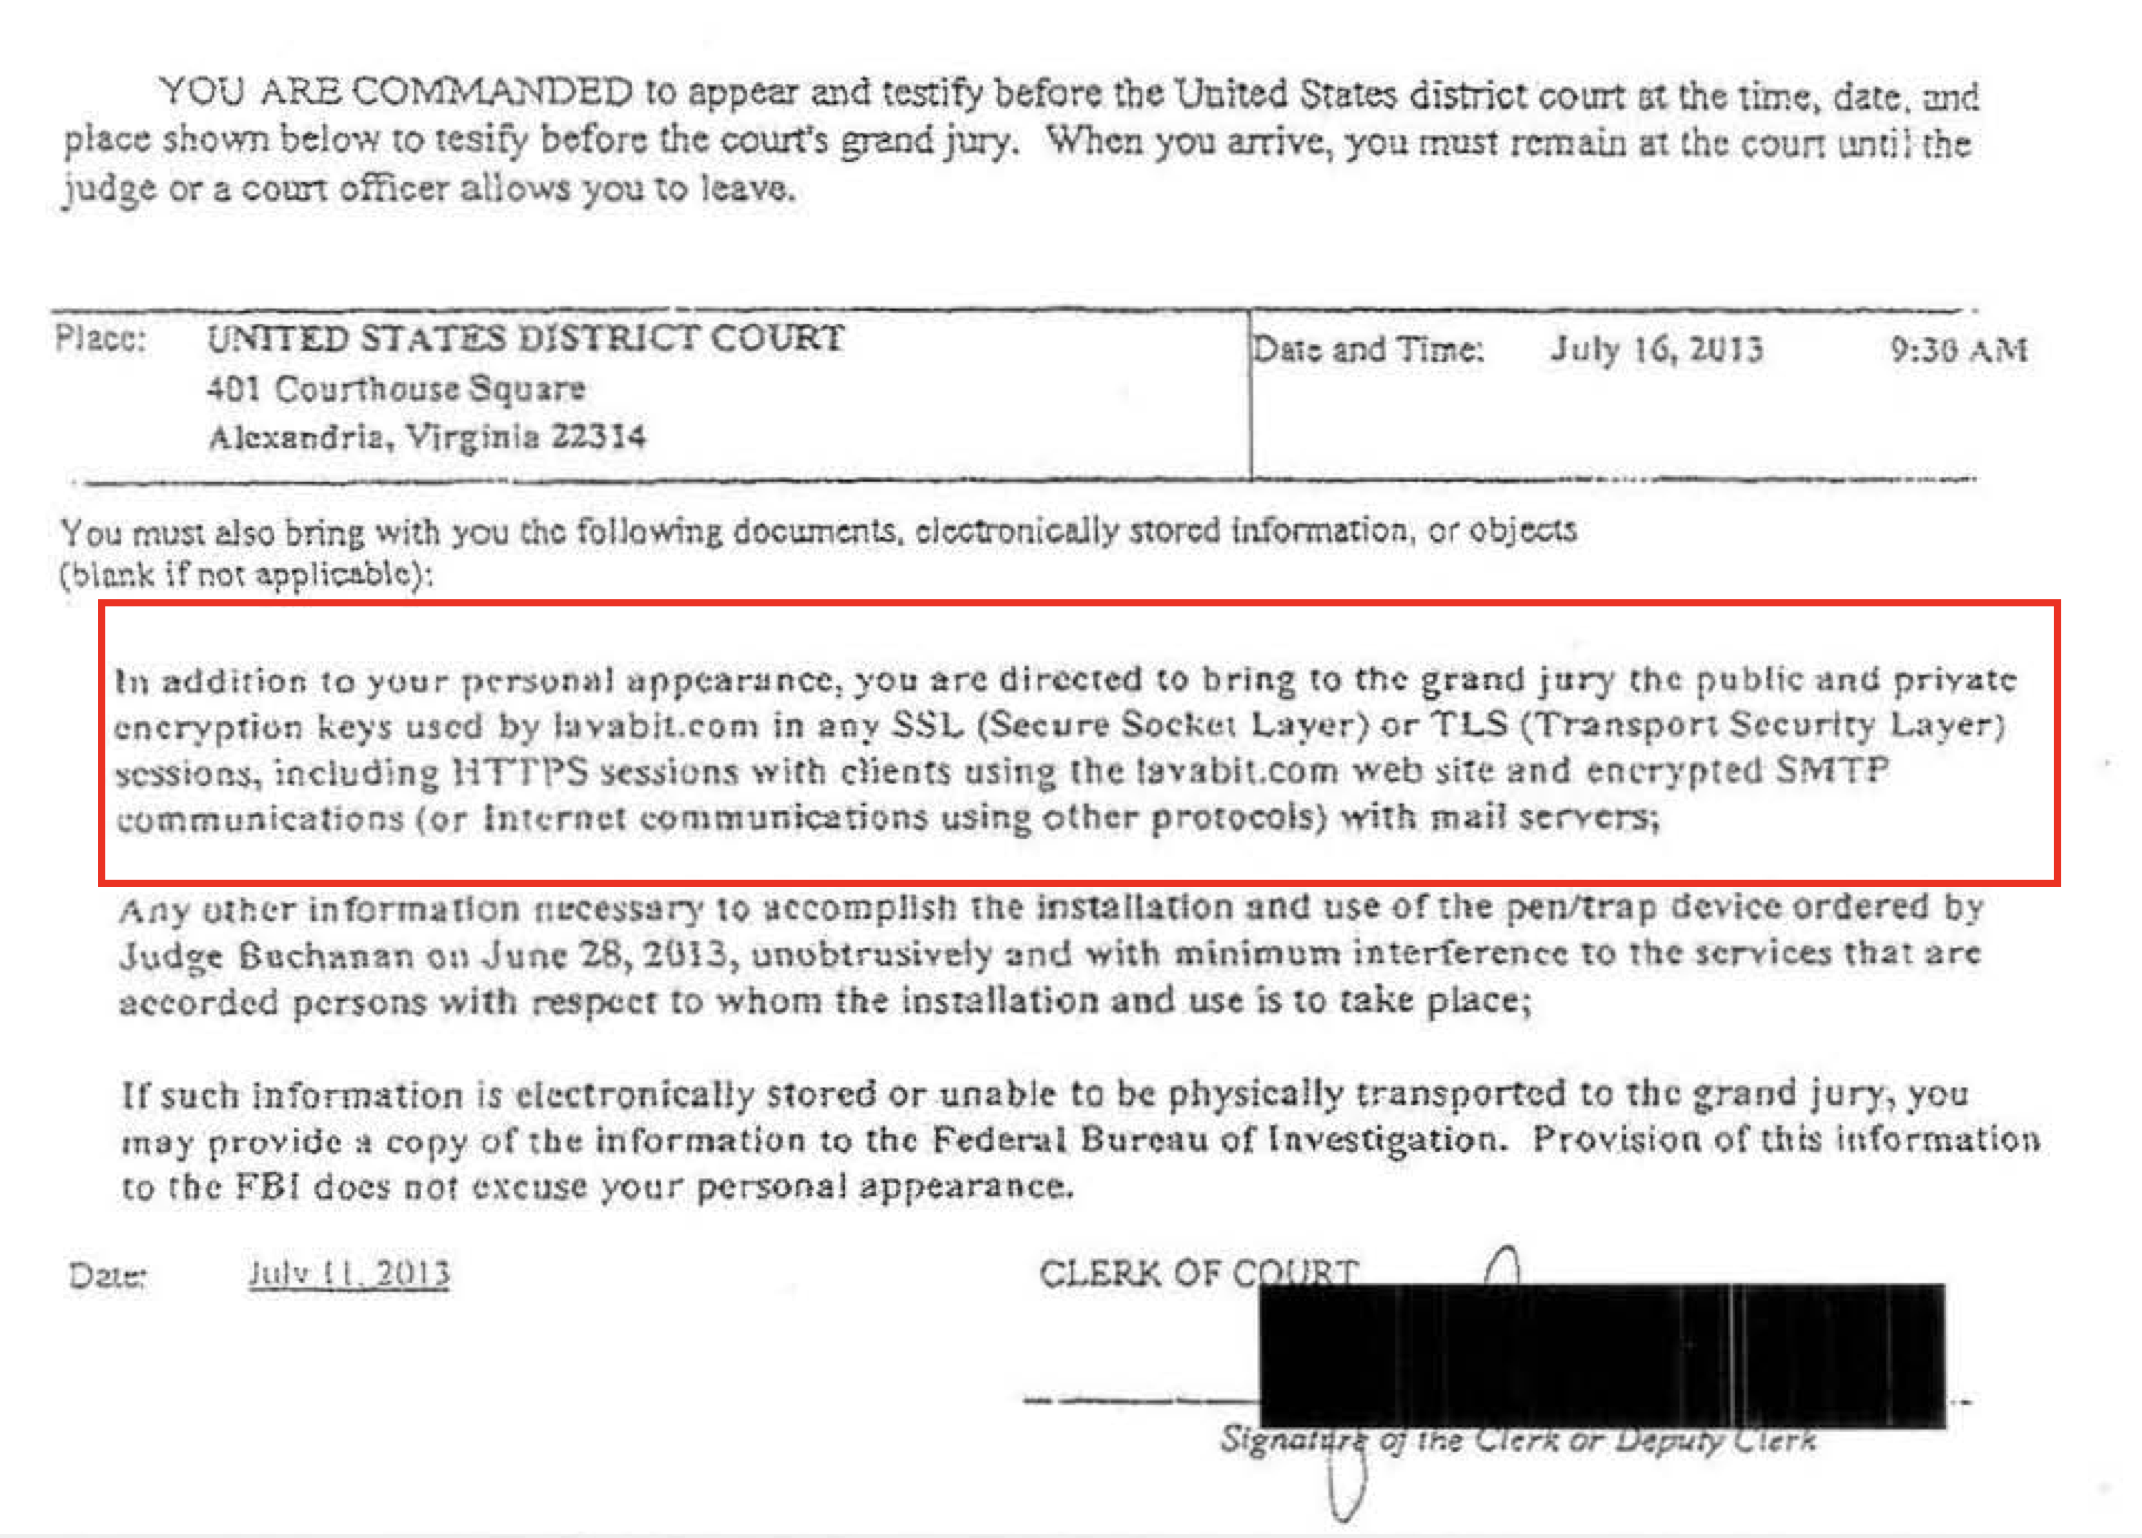
\includegraphics[scale=.3]{./lavabit-summons.png}

Lavabit was commanded to appear in court, and to bring all of their TLS, HTTPS, and SSL keys to present to the court. However, Ladar Levison chose to bring a blurry, illegible photo which he claimed to be the TLS key.

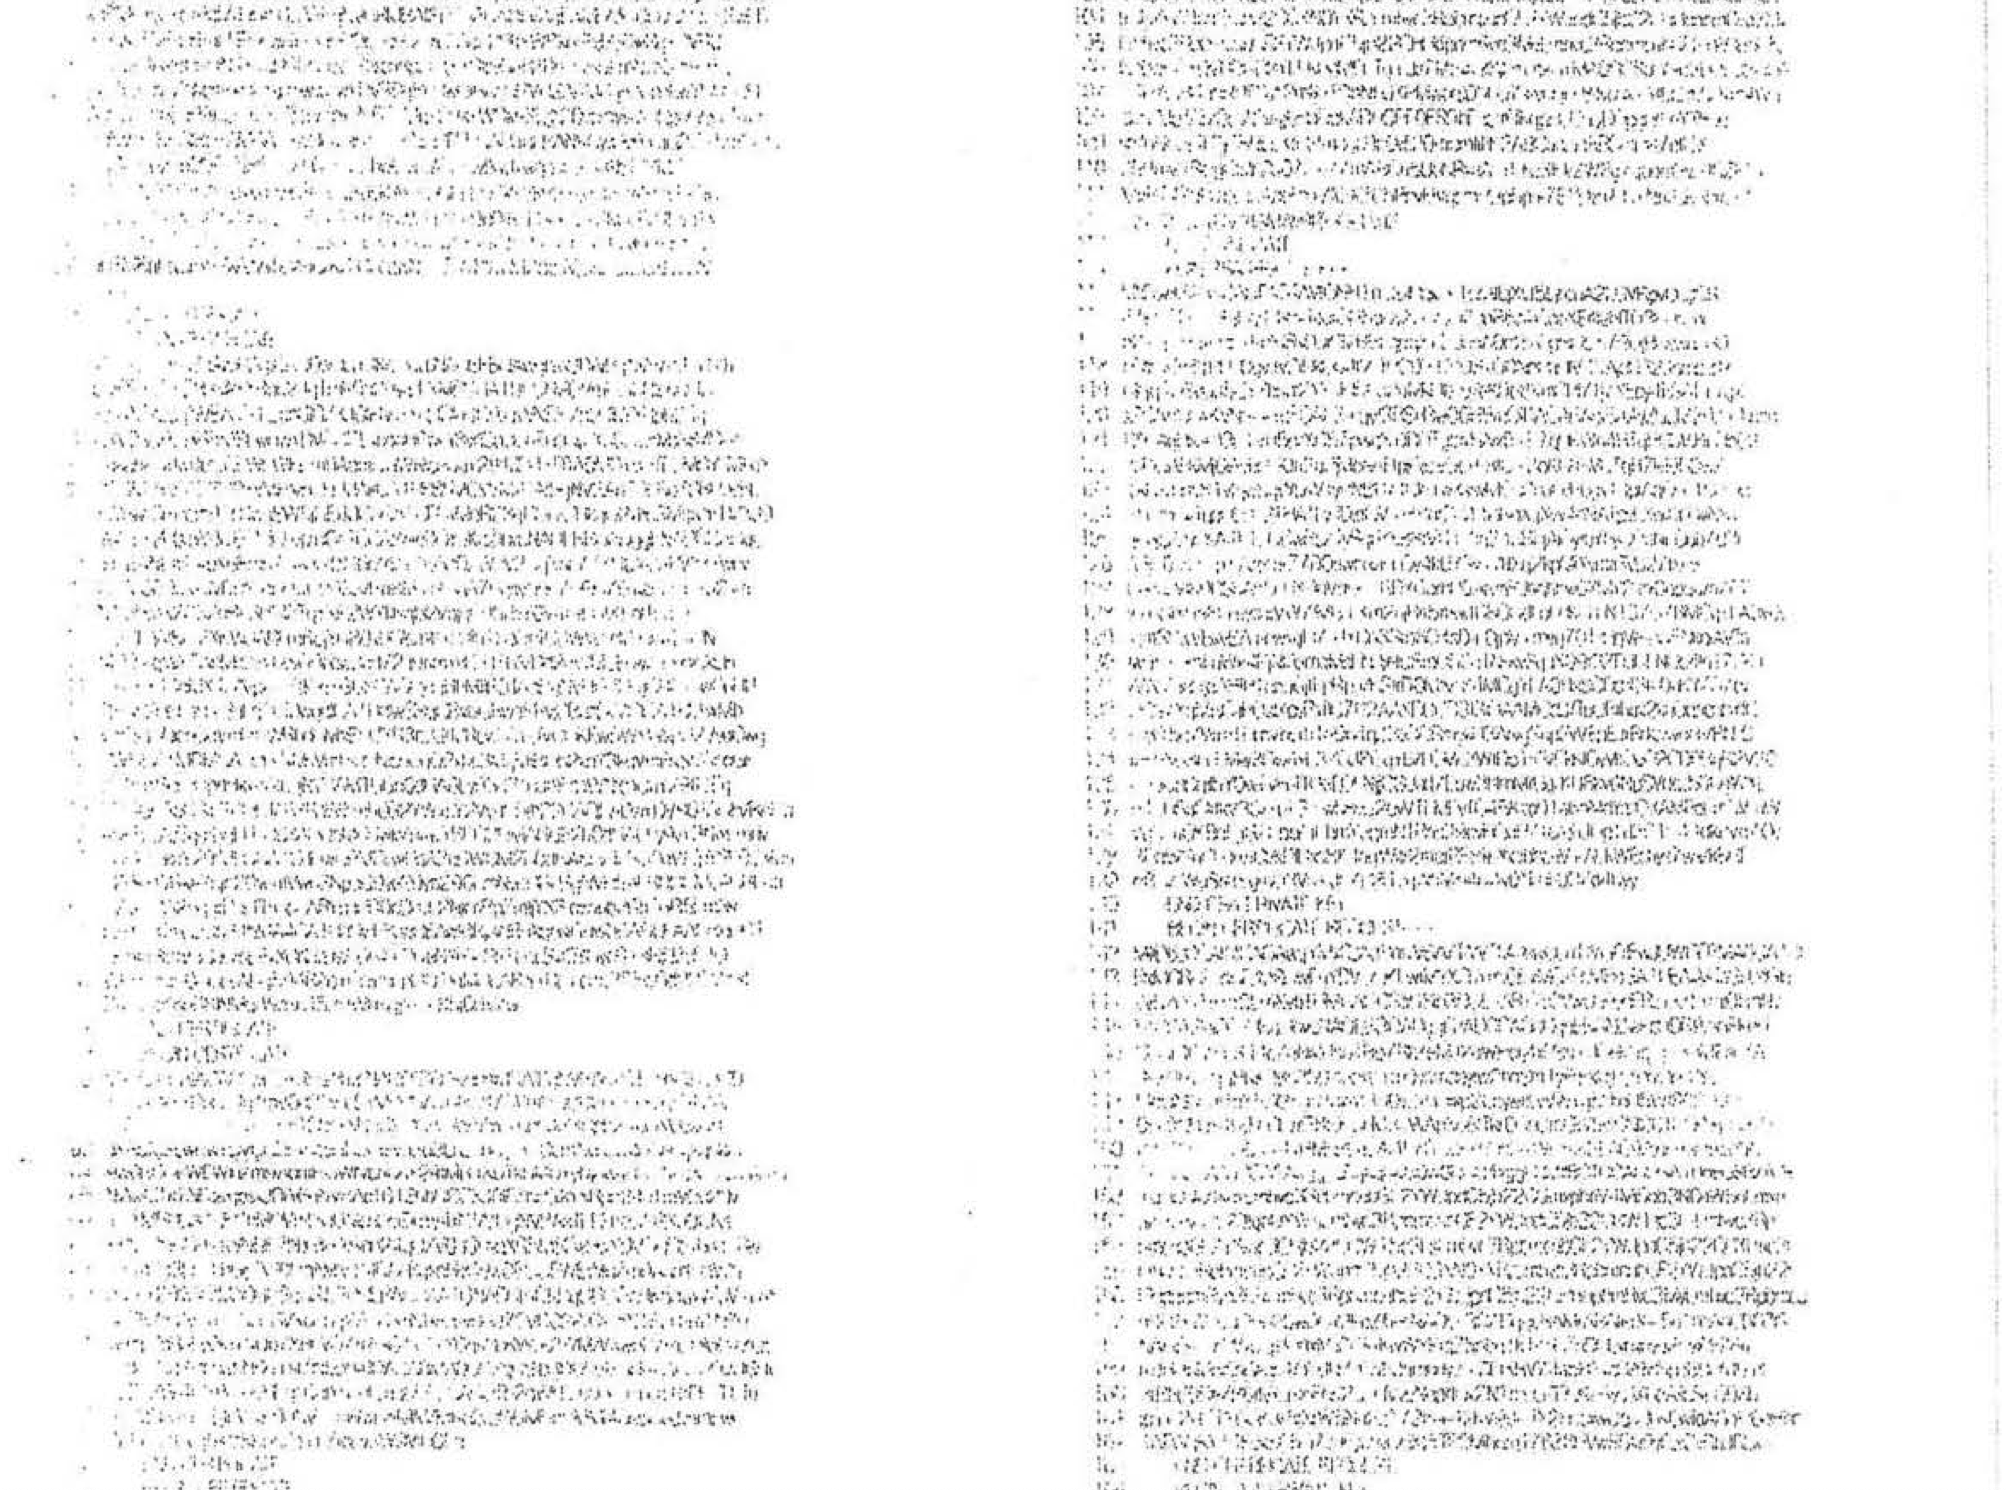
\includegraphics[scale=.3]{./lavabit-blurry-key.png}

Lavabit never gave up the key, and instead chose to end their business operations rather than violate the privacy of their customers around the globe. Politicians and the US government do not care about the individual's right to privacy. For example, here is a quote from former president Barack Obama:

"Because, if, in fact, you can’t crack that [encryption] at all, government can’t get in, then everybody is walking around with a Swiss bank account in their pocket – right? So there has to be some concession to the need to be able to get into that information somehow."


It is with this spirit that the US government has actually weakened encryption to make their job of spying easier. For example, in the 1990s, TLS 1.0 included options to weaken the protocol for US export control (browsers outside of the US were to request the weakened option). Even though these options are no longer required due to political shifts, there are still servers that respect the request. This lead to a series of attacks such as FREAK, logjam, and DROWN. 

\end{document}